\documentclass{article}
\usepackage{gvv-book}
\usepackage{gvv}
\usepackage{amsmath}
\usepackage{amsfonts}
\usepackage{tikz}
\usepackage{setspace}
\usepackage{gensymb}
\usepackage[cmex10]{amsmath}
\usepackage{amsthm}
\usepackage{mathrsfs}
\usepackage{txfonts}
\usepackage{stfloats}
\usepackage{bm}
\usepackage{cite}
\usepackage{cases}
\usepackage{subfig}
\usepackage{longtable}
\usepackage{multirow}
\usepackage{enumitem}
\usepackage{mathtools}
\usepackage{tikz}
\usepackage{circuitikz}
\usepackage{verbatim}
\usepackage[breaklinks=true]{hyperref}
\usepackage{tkz-euclide}
\usepackage{listings}
\usepackage{color}    
\usepackage{array}    
\usepackage{longtable}
\usepackage{calc}     
\usepackage{multirow} 
\usepackage{hhline}   
\usepackage{ifthen}   
\usepackage{lscape}     
\usepackage{chngcntr}
\usepackage{graphicx}
\usepackage{float}
\usepackage{multicol}
\usepackage[a4paper, left = 1.5cm, right = 1.5cm]{geometry}

\begin{document}

\begin{center}
\large
    \textbf{Samyak Gondane-AI25BTECH11029}
\end{center}
\date{}

\section*{Question}
The equation of the line through $(2, -4)$ and parallel to the X axis is \underline{\hspace{2 cm}}.

\section*{Solution}
Given: $\vec{p} = \myvec{2 \\ -4}$

\subsection*{Step 1: Direction and Normal Vectors}
The normal vector $\vec{n}$
\begin{align}
\vec{n} = \myvec{m \\ -1}\\
\vec{n} = \myvec{0 \\ -1}
\end{align}

\subsection*{Step 2: Dot Product Formulation}
Using the dot product form of a line:
\begin{align}
\vec{n}^T (\vec{X} - \vec{p}) = 0
\end{align}

Substitute:
\begin{align}
\myvec{0 & -1} \myvec{\vec{X} - \myvec{2 \\ -4}} = 0
\end{align}

\begin{align}
\Rightarrow \myvec{0 & -1}\vec{X} - \myvec{0 & -1}\myvec{2 \\ -4} = 0
\end{align}

\begin{align}
\Rightarrow \myvec{0 & -1}\vec{X} = -4
\end{align}


\subsection*{Final Answer}
\begin{align}
\boxed{\myvec{0 & -1}\vec{X} = -4}
\end{align}

\begin{figure}[H]
    \centering
    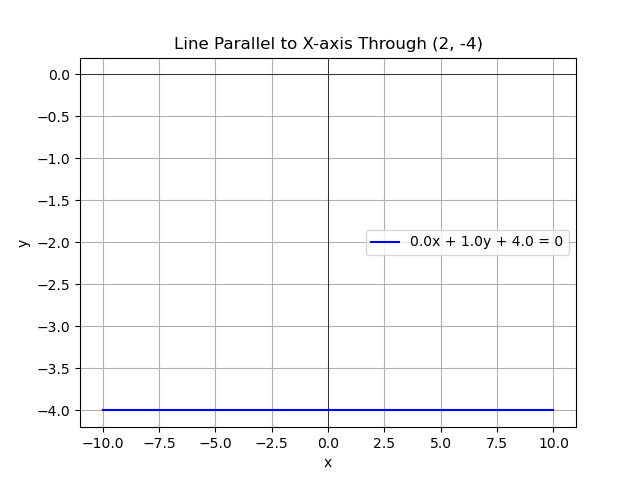
\includegraphics[width=0.5\linewidth]{./figs/Figure_1.png}
    \caption{}
    \label{fig:fig1}
\end{figure}

\end{document}